% !TEX root = ../main.tex
\iflatexml
\begin{figure}
    \centering
    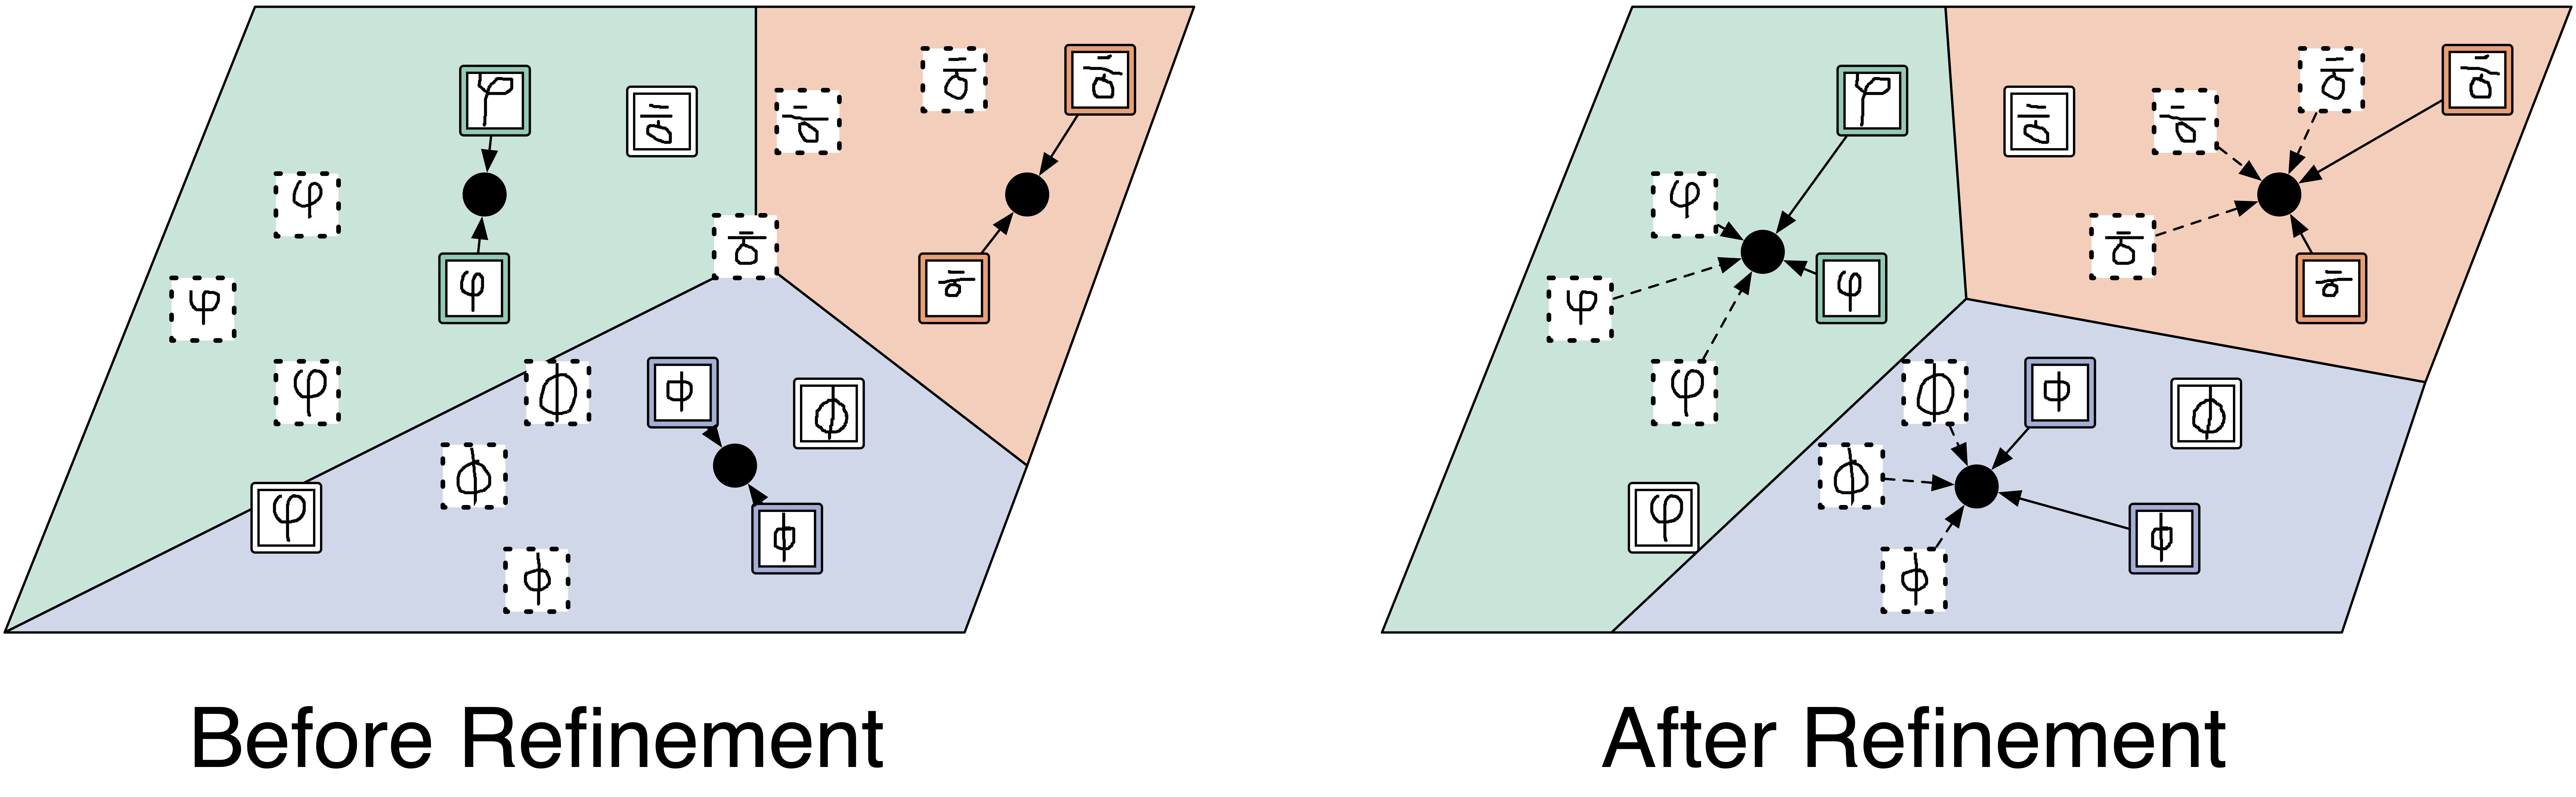
\includegraphics[width=6\textwidth]{figures/refinement_v4c.png}
    \caption{Left: The prototypes are initialized based on the mean location of the examples of the corresponding class, as in ordinary Prototypical Networks. Support, unlabeled, and query examples have solid, dashed, and white colored borders respectively. Right: The refined prototypes obtained by incorporating the unlabeled examples, which classifies all query examples correctly.}
    \label{fig:refinement}
\end{figure}
\else
\begin{wrapfigure}{r}{0.65\textwidth}
    \centering
    \vspace{-0.1in}
    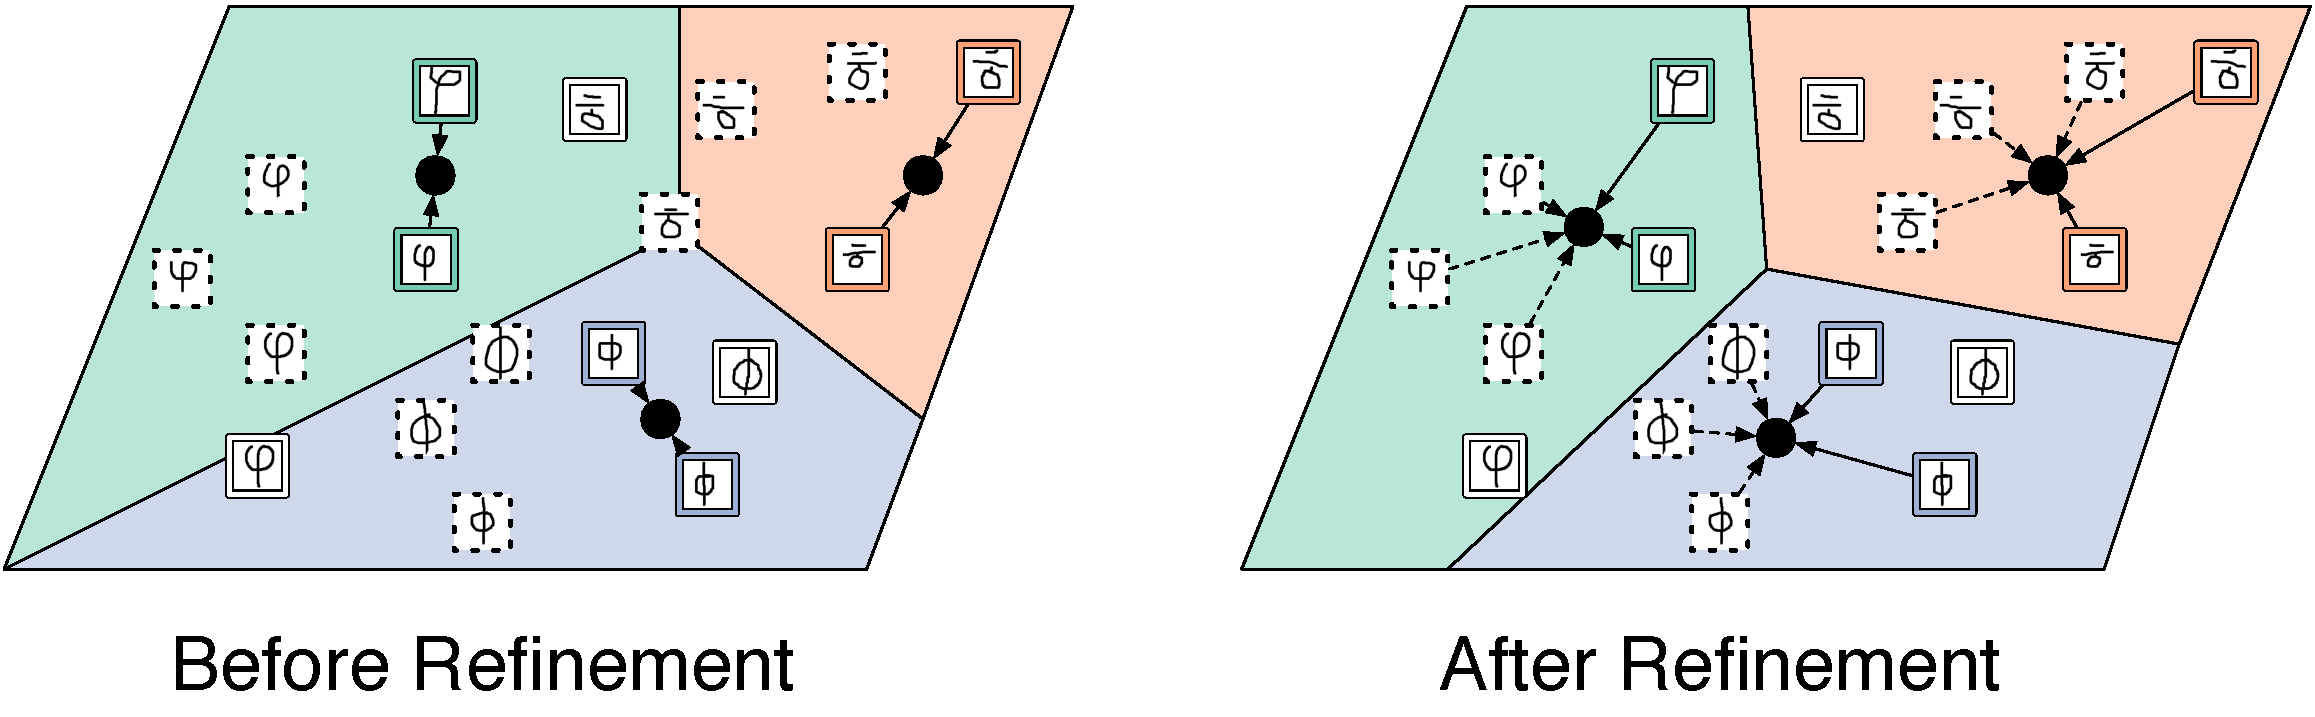
\includegraphics[width=0.6\textwidth]{figures/refinement_v4c.pdf}
    % \caption{Left: The prototypes are initialized based on the mean location of the examples of the corresponding class, as in ordinary Prototypical Networks. Support examples have solid colored borders, unlabeled examples have dashed borders, and query examples have white borders. Right: The refined prototypes obtained by incorporating the unlabeled examples. After refinement, all query examples are correctly classified.}
    \caption{Left: The prototypes are initialized based on the mean location of the examples of the corresponding class, as in ordinary Prototypical Networks. Support, unlabeled, and query examples have solid, dashed, and white colored borders respectively. Right: The refined prototypes obtained by incorporating the unlabeled examples, which classifies all query examples correctly.}
    \label{fig:refinement}
    \vspace{-15pt}
\end{wrapfigure}
\fi